% This is "sig-alternate.tex" V1.3 OCTOBER 2002
% This file should be compiled with V1.6 of "sig-alternate.cls" OCTOBER 2002
%
% This example file demonstrates the use of the 'sig-alternate.cls'
% V1.6 LaTeX2e document class file. It is for those submitting
% articles to ACM Conference Proceedings WHO DO NOT WISH TO
% STRICTLY ADHERE TO THE SIGS (PUBS-BOARD-ENDORSED) STYLE.
% The 'sig-alternate.cls' file will produce a similar-looking,
% albeit, 'tighter' paper resulting in, invariably, fewer pages.
%
% ----------------------------------------------------------------------------------------------------------------
% This .tex file (and associated .cls V1.6) produces:
%       1) The Permission Statement
%       2) The Conference (location) Info information
%       3) The Copyright Line with ACM data
%       4) Page numbers
%
% as against the acm_proc_article-sp.cls file which
% DOES NOT produce 1) thru' 3) above.
%
% Using 'sig-alternate.cls' you have control, however, from within
% the source .tex file, over both the CopyrightYear
% (defaulted to 2002) and the ACM Copyright Data
% (defaulted to X-XXXXX-XX-X/XX/XX).
% e.g.
% \CopyrightYear{2003} will cause 2002 to appear in the copyright line.
% \crdata{0-12345-67-8/90/12} will cause 0-12345-67-8/90/12 to appear in the copyright line.
%
% ---------------------------------------------------------------------------------------------------------------
% This .tex source is an example which *does* use
% the .bib file (from which the .bbl file % is produced).
% REMEMBER HOWEVER: After having produced the .bbl file,
% and prior to final submission, you *NEED* to 'insert'
% your .bbl file into your source .tex file so as to provide
% ONE 'self-contained' source file.
%
% ================= IF YOU HAVE QUESTIONS =======================
% Questions regarding the SIGS styles, SIGS policies and
% procedures, Conferences etc. should be sent to
% Adrienne Griscti (griscti@acm.org)
%
% Technical questions _only_ to
% Gerald Murray (murray@acm.org)
% ===============================================================
%
% For tracking purposes - this is V1.3 - OCTOBER 2002

\documentclass{sig-alternate-sigmod07}

\usepackage{tablefootnote}

\usepackage{hyperref}
\usepackage{cleveref}


\begin{document}
%
% --- Author Metadata here ---
%\conferenceinfo{ACM SIGMOD}{'07 Beijing, China}
%\CopyrightYear{2014} % Allows default copyright year (2000) to be over-ridden - IF NEED BE.
%\crdata{0-12345-67-8/90/01}  % Allows default copyright data (0-89791-88-6/97/05) to be over-ridden - IF NEED BE.
% --- End of Author Metadata ---
\makeatletter
\def\@copyrightspace{\relax}
\makeatother
\title{Detecting short-term anomalies in gas consumption using ARIMA and Robust Artificial Neural Networks}
%
% You need the command \numberofauthors to handle the "boxing"
% and alignment of the authors under the title, and to add
% a section for authors number 4 through n.
%
\numberofauthors{2}
\author{
% You can go ahead and credit any number of authors here,
% e.g. one 'row of three' or two rows (consisting of one row of three
% and a second row of one, two or three).
%
% The command \alignauthor (no curly braces needed) should
% precede each author name, affiliation/snail-mail address and
% e-mail address. Additionally, tag each line of
% affiliation/address with \affaddr, and tag the
% e-mail address with \email.
%
% 1st. author
\alignauthor
Marco De Nadai\\
       \affaddr{Universita' degli studi di Trento}\\
      \affaddr{Master's student}\\
       \email{marco.denadai@studenti.unitn.it}
% 2nd. author
\alignauthor
Maarten van Someren\\ 
       \affaddr{Universiteit van Amsterdam}\\
       \affaddr{Science Park 107}\\
       \affaddr{Amsterdam, The Netherlands}\\
       \email{m.w.vanSomeren@uva.nl}
}
\maketitle
\begin{abstract}

The focus of this paper is on building a robust outlier detection system, which relies on a hybrid Artificial neural network (ANN) and an Auto-regressive Integrated Moving Average (ARIMA) model. ARIMA is usually suitable for linear prediction and ANNs are suitable for non-linear prediction. It is proved that together they can model the complex non-linear relationship between weather forecast variables and the gas consumption. The system labels outliers, which can be reported to the building manager. He can further analyse and fix the HVAC system minimizing in this way the energy waste. 
The system is a 2-phase process where in the first one the short-term (hourly) gas consumption is forecasted thanks to a historical time-series, and in the second phase outliers are detected on the basis of deviations from expected (or forecast) value. 
Outliers are detected without the necessity of possessing the previously labelled examples, thanks to a very precise forecast with a RMSE error of $10$ $m^3$.

\end{abstract}

\keywords{Energy forecasting, Time series, Robust Artificial neural networks, ARIMA models, anomaly detection, outlier detection, gas consumption prediction, energy forecast}

\section{Introduction}

Energy consumption in buildings is one of the fastest growing sectors. Approximately $41\%$ of the total energy in Europe is consumed by buildings (households and services) \cite{Eurostat2013}. Studies and states' directives about minimizing energy consumption and using renewable energy increased steadily with the reduction of fossil fuels, the border frictions with eastern countries like Russia, and the increase of various environmental problems. With this in mind, the European union, with a recent directive \cite{Directive2009}, has the target to raise EU energy consumption produced from renewable resources to $20\%$, to reduce by $20\%$ the EU greenhouse gas emissions and to improve by $20\%$ the EU's energy efficiency. This means investments to re-qualify old buildings, new country laws, energy diagnosis, but also new efficiency systems from the used appliances.

Forecasting energy demands has become one of the major research field in the energy departments because it can help gas utilities but also companies and families. Gas utilities buy gas from pipeline companies on a daily bases, so they need to know the needs in advance to be competitive.  Companies and families have the aim of reducing the energy consumption and increase efficiency. \\
Lately, big companies like Google also have shown their interest in this new market, developing thermostats which automatically control the house climate basing the decisions on the schedule of the users. Nest, a company acquired by Google, declared that customers saved the 11.3\% of AC-related energy usage without compromising comfort \cite{GoogleNest2}, thanks to the automatic learning implemented in their thermostats. If on one hand the automatic thermostat program setting based on the people behaviour, can help them to save money, anomaly detection can decrease even more the energy consumption. These anomalies usually have a large impact on the final consumption and if caused by deficiency, they represents a huge and easy fixable problem. 

In this paper an automatic outlier detection system is proposed, where days/hours with abnormally high and low energy consumption are labelled and reported to the building manager. He can further analyse and fix the HVAC system minimizing the energy waste caused by the outliers. The outlier detection system presented is based on predictions made by a hybrid ARIMA-ANN, which can model linear and non-linear behaviour of the data with very reliable results, and a comparison between the predicted value/trend and the actual one to find outliers. 


\section{Background}

\subsection{What is an outlier}
An outlier, by definition \cite{hawkins1980identification}, is an observation which deviates significantly from other observations so that it creates suspicion that it was created by different dynamics. Despite this general definition, the more appropriate way of defining outliers is highly application-dependent, because even same scenarios may require different determinations of outliers. \\
In this paper, outliers are very closed related to the problem of time-series forecasting, since outliers are declared on the basis of deviations from expected (or forecast) value. In this context a value is considered as outlier because of its relationship to its related data (\emph{contextual} outlier \cite{aggarwal2013outlier} or conditional anomalies \cite{song2007conditional}). A sudden peak (\cref{fig:outlierTypes}) in a time-series is a \emph{contextual} outlier because its value is very different from the values of its adjacent items.\\
When a group of points are declared outliers, it is referred as \emph{collective} anomaly or outlier \cite{aggarwal2013outlier}. It first appear at a point and then it affects the values immediately next to it. After a while, this effect dies out, leaving the time-series to the normal behaviour. This scenario is usually challenging to detect.

 Outliers can have distinct main reasons: 
\begin{enumerate}
  \item Defective system (e.g. a defective heater in a room).
  \item Bad human behaviour (e.g. people who leave open the window in a room while the system is trying to heat it).
  \item Defective monitoring system, where the system monitors different values from the real one, due to a malfunction, computing process errors or a recording negligence. 
\end{enumerate}

In literature, outliers are also referred to as abnormalities, deviants, novelties or anomalies.

\begin{figure}[h!]
\centering
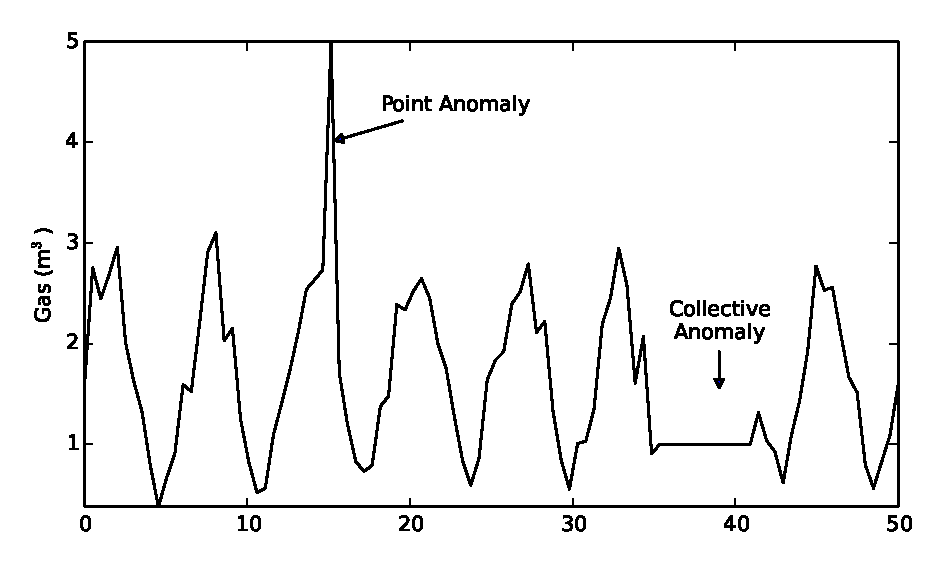
\epsfig{file=images/outlierTypes.eps, width=\columnwidth}
\caption{Different types of outliers. On the left an unusual data point is presented, on the right an unusual pattern of changes can be recognized if compared to the other days shape.}
\label{fig:outlierTypes}
\end{figure}


\subsection{Artificial Neural Networks}
Artificial Neural Networks (ANNs) were originally developed to mimic the brain functionality. There is not a widely accepted definition but by \cite{bishop1995neural}: ''A neural network is a circuit composed of a very large number of simple processing elements that are neurally based. Each element operates only on local information. Furthermore each element operates asynchronously; thus there is no overall system clock. '' 
From \label{fig:ANN}, it is possible to see a fully connected ANN with five inputs, 3 neurons on the hidden layer (so called because the ANN is like a black-box) and one output. The inputs are also called features and they represent the characteristics to describe the output. The hidden neurons will map this relation. Each connection has an activation which represents the importance (weight) of the connected neuron. ANNs with at least 1-hidden layer can map non-linear relations.

The hidden neurons are usually represented with logistic sigmoid units, which internally calculates the sigmoid function of the inputs, but also with hyperbolic tangent. Recent findings argued that rectifier units seems to be more biologically plausible \cite{glorot2011deep} and they also seem to perform better in ANNs. 
\begin{figure}[h!]
\label{fig:ANN}
\centering
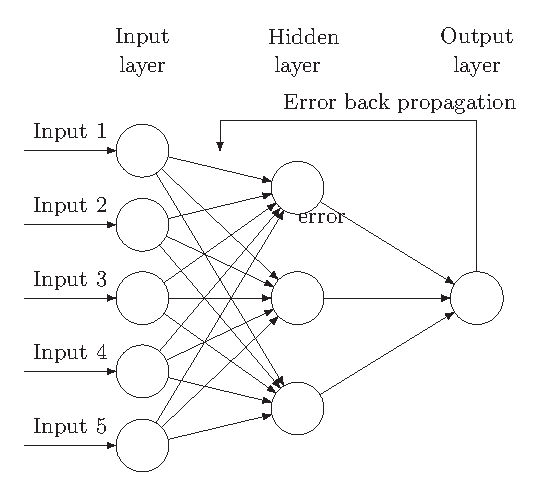
\epsfig{file=NN2.eps, width=\columnwidth}
\caption{Artificial neural network with \emph{Backpropagation}. Example with 5 inputs, 3 hidden neuron in the first hidden layer, and one output (in the case of this paper, the gas consumption value).}
\end{figure}

The ANNs are commonly applied with the \emph{Stochastic Gradient Descent} algorithm, which tries to find the right weights of each connections to have the right output value. It is usually combined with the \emph{Backpropagation} algorithm which calculates the error in the output layer and then back-propagates it to the previous layers in order to adjust the weights \cite{rumelhart1985learning}. More information can be found in \cite{bishop2006pattern}.

Nowadays, ANNs are the state of the art technique of many applications.


\subsection{Autoregressive models}
Let $X_1, X_2, \ldots X_t$ be the values in an univariate time-series. In the \emph{Auto-Regressive Moving Average} model, the value of $X_t$ is defined in terms of the values of the last window of length $p$ and $q$ moving average terms.
\begin{displaymath}X_t =  \sum_{i=1}^p \varphi_i X_{t-i} + \sum_{i=1}^q \theta_i \varepsilon_{t-i} + c + \varepsilon_t.\end{displaymath}
The left-hand part is called auto-regressive part, because it depends on the previous (lagged) values $X_{t-1}, X_{t-2}, \ldots X_{t-p}$, the right-hand part is called moving average because the error at time $t$ is the linear combination of the previous errors $\varepsilon_{t-1}, \varepsilon_{t-2}, \ldots, \varepsilon_{t-q}$. \\
These methods are applied to \emph{stationary} time-series, so called when the mean, variance and autocorrelation structure do not change over time. Sadly, many time-series have seasonal effects or trends. In particular, random walks,
which characterise many types of series, are non-stationary. Differencing the data-points can often transform a non-stationary time-series into a stationary one. Based on the Box-Jenkins models of the $1970s$, ARIMA models differentiate where series with deterministic trends should be differenced first, then an ARMA model applied. ARIMA models are usually mentioned as $ARIMA (p, d, q)$, to show the ARMA parameters and the $d$ order of difference.ARIMA models are also capable of modelling a wide range of seasonal data. 
\begin{displaymath}
\operatorname{ARIMA}(p,d,q) (P,D,Q)_m
\end{displaymath}
where $m$ is the number of periods per season. The upper-case notation is used for the seasonal parts of the model, and the lower-case notation for the non-seasonal parts of the model.

The choice of the parameters $p$, $d$, $q$ is highly application dependent and it relies on theory that is beyond the scope of this paper. More information can be found in \cite{rousseeuw2005robust}.


\section{Related work}
 Since in this paper outliers are declared on the basis of deviations from expected (or forecast) value, this section is divided in related work in forecasting and outlier detection.


\subsection{Outlier detection}
Outlier detection system is a wide area from introduction detection systems to fraud detection systems, from law enforcement systems to earth science anomaly detection systems.\\
Outlier detection can be supervised, when available data is labelled indicating previously known examples of anomalies, semi-supervised, where only example of normal data or anomalies are available, or unsupervised, where previous examples of interesting anomalies are not available. Typically most of the unsupervised outlier mechanisms use a measure of \emph{outlierness} of a data point, such as sparsity of underlying region, nearest neighbour distance or the fit to underlying distribution \cite{aggarwal2013outlier}. In these cases a data-point is unusual due to one or more variables rather than a specific one (like in the supervised methods).

In energy consumption outlier detections, literature is usually based on the Gaussian error theory, stating that when the measurement accord with normal distribution, the probability that the residual falls in three times the variance is more than $99.7\%$. Therefore the residuals falling outside it, can be considered outliers. 
In \cite{ferdowsi2013neural} the author further improved this system considering a rolling window median which seems to improve the results when the distribution is not fixed. Supervised methods are usually based on classifications using trees, ANNs and other different algorithms, thanks to the possession of previous examples of anomalies. In energy consumption field unsupervised methods are usually based clustering, where an algorithm tries to find similarities between points/trends and cluster them into groups, calculating the distance between them. A cluster is considered good when the intra-cluster distance is minimized and the intra-cluster distance is maximized. Popular methods in this group are $k$-means, one-class SVM and self-organizing maps. Despite this can be true, they are very difficult to apply in time-series data and the results are not usually excellent. For this reason in this paper a prediction algorithm will be built, where outliers are declared on the basis of deviations from expected (or forecast) value. The more the predictor will be accurate, the more it will detect abnormal data points.


\subsection{Forecasting}
Traditionally, several techniques have been used for energy use forecasting, but it is needed to differentiate between short-term, medium-term and long-term energy forecasting. The former usually refers to prediction with a horizon of hours or days, the second refers to weeks, the latter refers to monthly or annual horizon. Long-term forecasting usually deals with data that rarely presents significant distortions and irregularities, so they have a small effect on the overall value. On the contrary, short-term forecasting has to deal with irregularities and sudden changes of the values (due to weather changes, human behaviour, etc.). 

There are essentially five types of prediction models \cite{zhao2012review}: Engineering methods, Statistical methods, Artificial Neural networks, Support Vector Machines and Grey models. Engineering methods use physical principles to calculate thermal dynamics and energy behaviour of the building, Statistical methods build empirical models to apply a regression to time series of values, Neural networks try to predict energy using an artificial intelligence network of interconnected neurons, Support vector machines are based in a machine learning algorithm and Grey models apply a mixture of the models. All the principal methods are extensively reviewed in \cite{zhao2012review} and \cite{hippert2001neural}. 

Several techniques have been traditionally applied for energy use forecasting, and among the statistical methods Kalman filtering and ARIMA/ARMAX time-series techniques are the most famous. 

The first reports about applications of Artificial Neural Networks (ANNs) were published in the early 1990's \cite{czernichow1996short}. Since then the number of publications increased steadily. Kalogirou et la. \cite{kalogirou2006artificial} used back propagation neural networks to predict the required heating load of 225 buildings, Ekici and Aksoy used the same model t predict building heating loads in three-buildings. Nizami and Al-Garni \cite{JaveedNizami19951097} tried a simple feed-foward NN and related the electric energy consumption to weather data and population, Taylor and Buizza \cite{taylor2002neural} used an ANN with weather data (51 variables) to predict load of 10 days ahead. Gonzales \cite{gonzalez2005prediction} built an ANN to predict hourly energy consumption.
Some researchers tried to specialize the ANNs: Neto and Fiorelli \cite{neto2008comparison} compared generic ANNs with working days ANNs and week-end ANNs, Lazzerini and Rosario \cite{d2012neural} specialized them to predict electric lighting with weather data. 

Some researchers tried also to apply a hybrid model to increase the performance of the ANN. One example above all is \cite{zhang2003time} which applied a hybrid ARIMA and neural network model to forecast electricity use, another one is \cite{khashei2010artificial} who improved the previous one. This paper is based also on his work.

Until now only electric forecasting was presented, because the majority of the existing forecasters are related to electric forecasting. There are only few of them are about natural gas forecasting: Brown et al.\cite{brown1995development} built one of the first predictor for natural gas consumption and Khotanzad et al \cite{khotanzad2000combination} developed a two stage system ANN with very good results.

Even if ANNs might outperform traditional methods, the researchers are not still convinced about the results of the ANNs in this field. Nevertheless it is also stated that ``a significant portion of the ANN research in forecasting and prediction, lacks validity" \cite{adya1998ective} and that most of the papers seems misspecified models that had been incompletely tested (no standard benchmarks, no synthetic data, etc.) \cite{hippert2001neural}. This paper will try to avoid these mistakes.

It needs also to be pointed that ANNs are \emph{multi-step ahead} forecasters, while Auto-Regressive methods are potentially useless in long ahead data-points.

\section{Proposed solution}
\label{sec:proposedSolution}

As stated before, in this paper an regression algorithm is proposed where outliers are declared on the basis of deviations from expected (or forecast) value.

A time-series is a sequence of data-points typically measured at successive points of a uniform time interval $t$ (\cref{eq:timeseries}).
\begin{equation}\label{eq:timeseries}\left\{x(t_0), x(t_1), \ldots x(t_i), x(t_{i+1}) \ldots \right\}\end{equation}
where $x$ is the value and $t$ the time.

Time-series forecasting is about predicting future values given past data (\cref{eq:forecast}). 
\begin{equation}\label{eq:forecast}\hat{x}(t+s) = f\left(x(t), x(t-1) \ldots \right) \end{equation}
where $s$ is the step size. A \emph{multivariate} time-series is a $(n\times1)$ vector of $n$ time-series variables.

It can be seen that in academic and industry research, linear regression-based systems are the standard ``de facto" of energy forecasting and in recent works this problem is treated by combining weather forecast data. However, this relationship is clearly non-linear \cite{hippert2001neural}. Consequently, even if some papers have acceptable results with measured datasets, these systems cannot adequately capture the relationship in all the situations and data. Since ANNs are the state of the art technique of many machine learning problems where there are complex non-linear hypothesis, the proposed solution is composed by a \textit{multilayer feed-foward} neural network with \textit{backpropagation}. 


\subsection{Experimental data}
The energy consumption datasets used are collected by Ebatech in different buildings of the Hogeschool van Amsterdam. These buildings are located in Amsterdam, the capital city of The Netherlands. This city has a maritime climate similar to England, strongly influenced by the North Sea. Winters are fairly cold and summers are rarely hot for the european standards. Amsterdam is characterized by the common presence of rain and wind and the weather conditions vary frequently.\\
Ebatech collected different types of features in each buildings, with different granularity. For this project three buildings are used: \textit{HvA 740 - NTH}, \textit{Hva 882 - WBW} and \textit{Hva 761 - KMH}. In these buildings the company collected the energy consumptions, the gas consumptions as other variables.

\begin{table}
\centering
\caption{Buildings used}
\label{tab:dataset}
\begin{tabular}{|c|c|l|} \hline
Building name&Date interval&Number of rows\\ \hline\hline
HvA 740 - NTH & 01/2008 - 03/2014 & $54.725$\\ \hline
Hva 761 - KMH & 01/2008 - 03/2014 & $54.744$\\ \hline
Hva 882 - WBW& 01/2008 - 03/2014 & $54.647$\\ \hline
\end{tabular}
\end{table}

The weather data was collected by KNMI\footnote{Koninklijk Nederlands Meteorologisch Instituut http://www.knmi.nl} in Schipol, the Amsterdam airport 16 km far from the tested buildings. The available data consists in over 21 variables hourly collected. The proposed solution only uses few of them, as explained in the \cref{sec:predictor}, and they are used as forecast values: the measured weather conditions are linked to the previous hour of energy consumptions. It is necessary to consider that there will be an error in the built model, since the weather data is collected in a different location from the buildings positions and in practice the error will be larger than those obtained in this simulation, due to the effect of the weather forecast uncertainty \cite{douglas1998impacts, ranaweera1996effect}. The advice is to keep it in mind before applying the methods contained in this paper with days forecasting.


\subsubsection{Data analysis}
\label{sec:dataAnalysis}

The available dataset is conform to the nine characteristics of a good dataset as outlined by to Few \cite{few2009now}:
\begin{description}
\itemsep0em
  \item[Volume] As demonstrated in \cref{tab:dataset}, the dataset seems adequately large to train an ANN and test the results.
  \item[Historical] The dataset covers a very large period ranging more than 5 years, allowing to see similar patterns even with different yearly/seasons behaviour (one year could be different from another one for external factors like weather or building use). 
  \item[Consistent] The dataset of the selected buildings and for the variables that will be used, is consistent.
  \item[Multivariate] In this paper a \emph{multivariate} time-series problem is considered and the dataset is composed by more than 50 variables, measuring the different behaviours of the buildings and the weather.
\item[Clean-Atomic] The dataset is clean and atomic after the cleaning process (\cref{sec:cleaning}).
\item[Clear] The dataset of the selected buildings and for the variables that will be used, is clear. The only problems were found on the not used variables: although they could be very useful, it was not possible to contact the buildings energy managers in order to understand them, for this reason they were excluded.
\item[Richy Segmented] This principle is not considered in this paper, but the dataset can be segmented in several meaningful segments like gas consumption, electric consumption, water consumption, number of people using the buildings, etc.
\end{description}

The gas consumption data is highly seasonal: daily and weekly cycles are quite perceptible, as it can be seen from \cref{fig:monthlyTGas} and \cref{fig:dailyBehaviour}. From the latter the weekly behaviour is clear: the last two days of the week (Saturday and Sunday) are completely different from the others and Monday seems a bit different from the rest of the days. Everyday, around 4:00-5:00 AM, the system seems to react turning on the heating system, where in the previous hours of the night it seems only keeping a minimum temperature. The system reveals us that after a couple of hours, it decreases the consumption again.
In \cref{fig:monthlyTGas} the Temperature has a clear daily/hourly relation with the gas consumption while in \cref{fig:monthlyGasElectr} the electric consumption is shown to be very smoothed and more regular than the gas one.


\begin{figure}[h!]
\centering
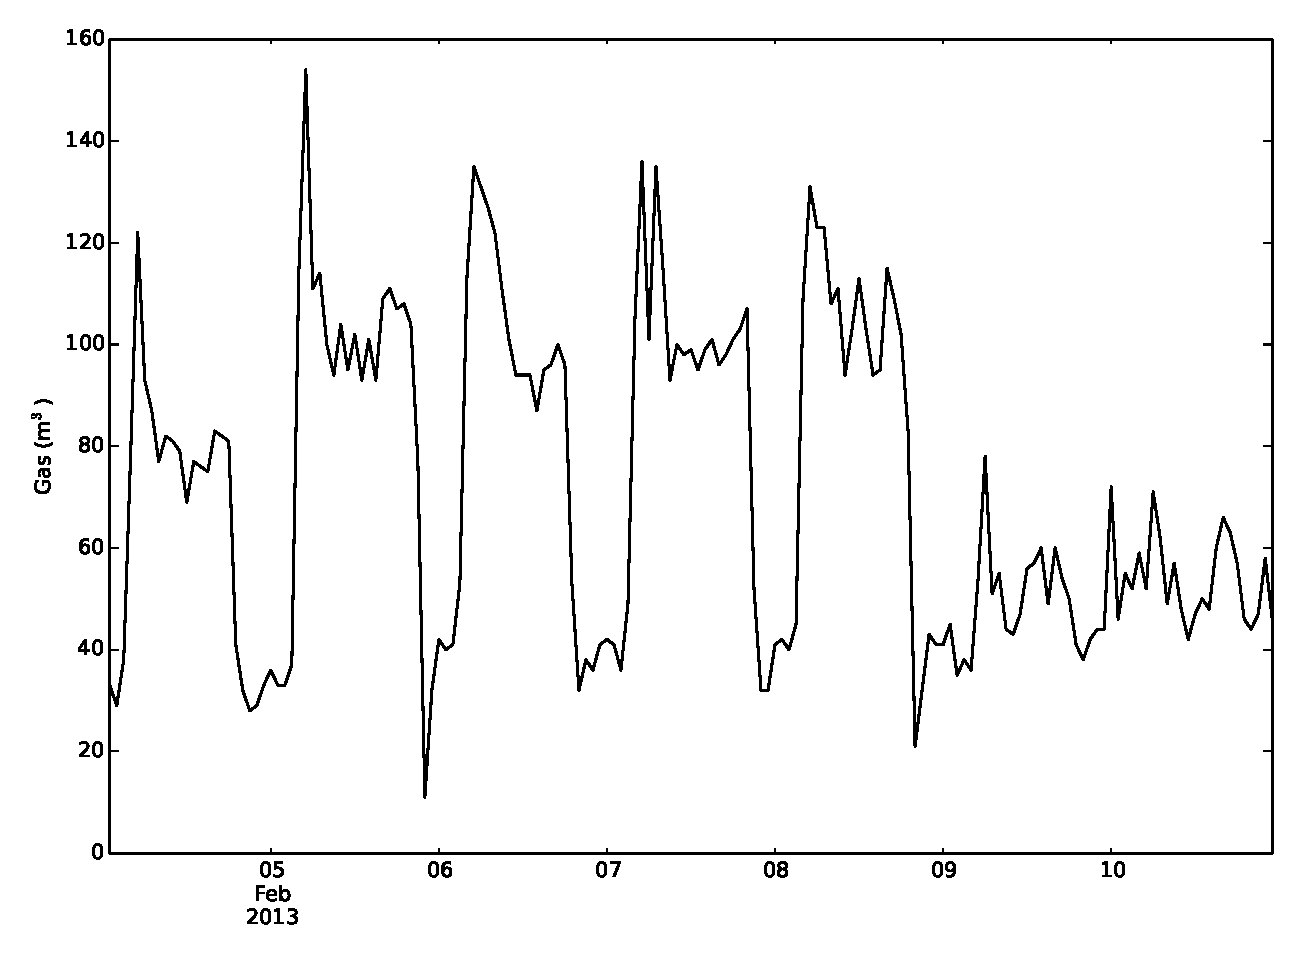
\epsfig{file=images/dailyBehaviour.eps, width=\columnwidth}
\caption{Typical weekly and daily gas consumption behaviour. The weekly pattern can be noticed by observing that the last two days of the week (Saturday and Sunday) have a completely different shape than the others. During the week, the daily behaviour is very similar, with one peak around 4:00-5:00 AM.}
\label{fig:dailyBehaviour}
\end{figure}

\begin{figure}[h!]
\centering
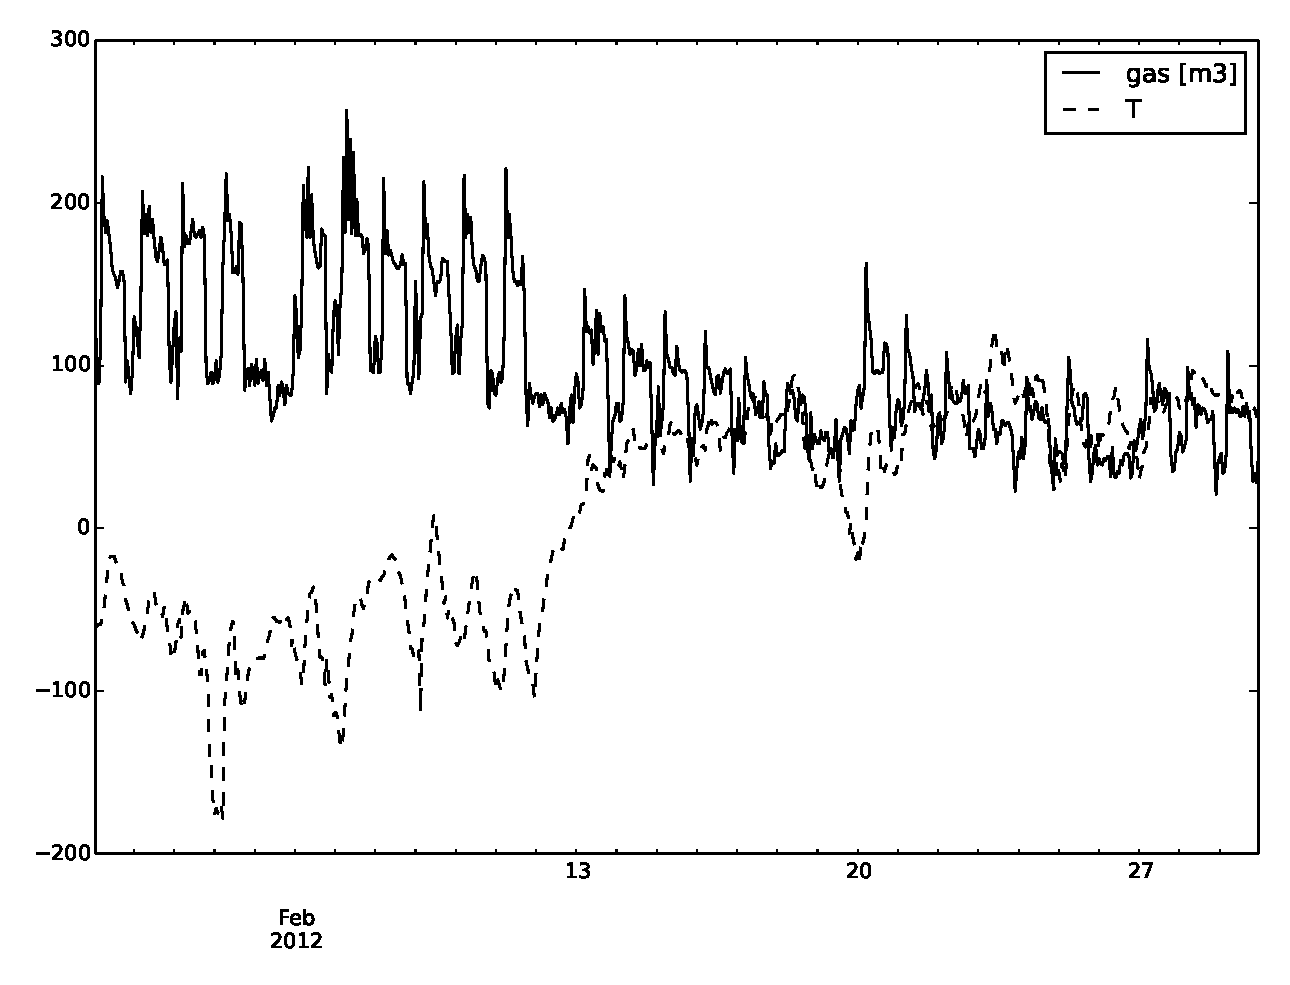
\epsfig{file=images/monthlyTGas.eps, width=\columnwidth}
\caption{Typical monthly gas consumption behaviour and its relation with the temperature}
\label{fig:monthlyTGas}
\end{figure}

\begin{figure}[h!]
\centering
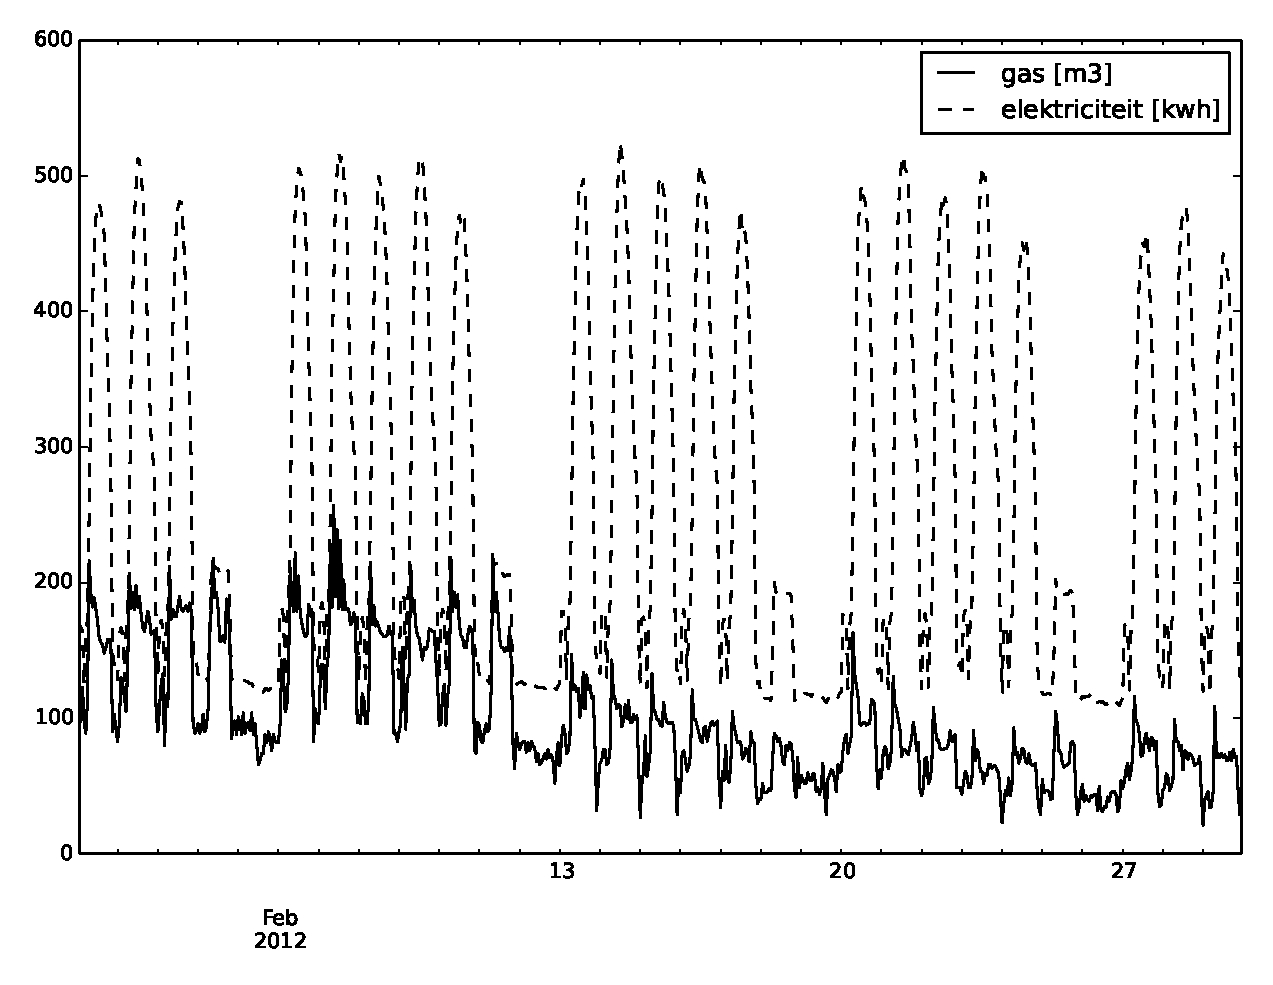
\epsfig{file=images/monthlyGasElectr.eps, width=\columnwidth}
\caption{Relation between electric and gas consumption}
\label{fig:monthlyGasElectr}
\end{figure}


\subsubsection{Data cleaning}
\label{sec:cleaning}
The data was presenting some irregularities like repeated and missing data-points. Although the first one may not influence the performance of the ANN, it could lead to problems when other algorithms are used (like ARMA in this paper). Repeated data-points were deleted keeping only the last one, while missing data-points were reconstructed by linear interpolation. Cubic and spline interpolation were also considered but the performance was heavly affected by these methods.


\subsection{Artificial neural network forecaster}
\label{sec:predictor}

Time-series are characterized by more or less complex dependencies:
\begin{description}
\itemsep0em
  \item[Known] dependencies like date-time dependencies.
  \item[Hidden] dependencies like the behaviour of the HVAC system (when it starts, when it raises the temperature etc).
  \item[Short/long-term] dependencies between variables.
\end{description}
Data scientist and experts are focused in known dependencies while the proposed ANNs will be focused on the hidden ones.
The short/long-term dependency is realized by a moving window containing a ``memory" of the previous states for the interesting variables, using a \emph{Tapped delay line memory} \cite{mozer2007neural}. These memories form a new set of states \begin{displaymath}\left\{\bar{x}_1(t), \bar{x}_2(t), \ldots \bar{x}_n(t)\right\}\end{displaymath} from the original states \begin{displaymath}\left\{x(1), x(2) \ldots x(n)\right\}\end{displaymath}where $\bar{x}_i(t) = x(t - i + 1)$. The window types will be explained later in this section. 

Since the value to predict is time dependent, the first element to consider is adding the time feature. Energy consumption depends on the hour of the day but also on the day of the week and the seasonality of the year (month and day of the year) (as explained in \cref{sec:dataAnalysis}, \cref{fig:monthlyTGas} and \cref{fig:dailyBehaviour}). The day of the week is a number from $0$ to $6$, where $0$ is Monday and 6 is Sunday. Since the behaviour of the holidays were considered similar to the weekends (particularly similar to Sundays), a function encoded all the holidays as weekend days\footnote{Thanks to an Open source dutch week-end list \url{https://github.com/PanderMusubi/dutch-holidays}}. The day of the year is a number between $0$ and $366$, where the first one is the first of January. All these date-time features by means of their sine and cosine values as usual reported in literature \cite{ohlsson1994predicting, dodier2004statistical, gonzalez2005prediction}. This transform the time component in a cyclic feature that spans a fixed length (a single day for the hour) and it is bounded in $[-1,1]$.

Another added feature was the current system load, which is the energy consumption at the $k$ state when the load at $k+1$ needs to be predicted. This was believed to be an important measure to find the building usage and the holidays.

There are many factors that affect the energy needs of buildings. These factors can be divided in three main groups namely the \emph{physical environmental}, the \emph{artificial designing parameters} and the \emph{human thermal discomfort}. The first is composed of weather related parameters like outdoor temperature, wind speed, solar radiation, etc. The \emph{artificial designing parameters} are related to the building construction: transparency ratio, orientation, etc \cite{ekici2009prediction}, but these variables were unavailable in the dataset. The \emph{human sensation of thermal discomfort} is correlated not only to the temperature, but also to other variables such as relative humidity, irradiation and wind speed. Even if all these data was available, the only significant weather variables found, were the temperature and the wind speed.

The system consumption was believed to be related to the difference of the outdoor temperature between two instants (\cref{eq:differenceT}), representing a positive/negative change of the external environmental conditions.
\begin{equation}\Delta T_{k+1}=T_{k+1} - T_{k}\label{eq:differenceT}\end{equation} where $T_{k+1}$ is the predicted temperature for the period $k+1$ and $T_k$ is the value measured in the instant $k$. It needs to be noted that the real behaviour of the system was unknown, so it was not possible to know if this change would have an immediate effect on the HVAC system and/or its reaction time.

Gas usage has a daily cycle but there are also secondary weekly and annual cycles that the ANN may not be able to capture. Gas usage $u(t)$ is defined as \begin{displaymath}u(t) = s(t) + f(t) + r(t)\end{displaymath} where $s(t)$ is the seasonality at time $t$, $f(t)$ is the trend and $r(t)$ is called \emph{remainder}, irregular component or difference. The time-series was analysed by the STL decomposition by LOESS \cite{cleveland1990stl}(\cref{fig:STL}), which decomposes a time series into seasonal, trend and irregular components by an additive method. Since the ANN is interested in the \emph{remainder} and the trend can be found from the historical part, the daily, weekly and yearly remainders were added as feature. For the same reason also the Temperature, the wind speed and the electric consumption was decomposed by the STL decomposition, resulting in stationary time-series added in the input.

\begin{figure}
\centering
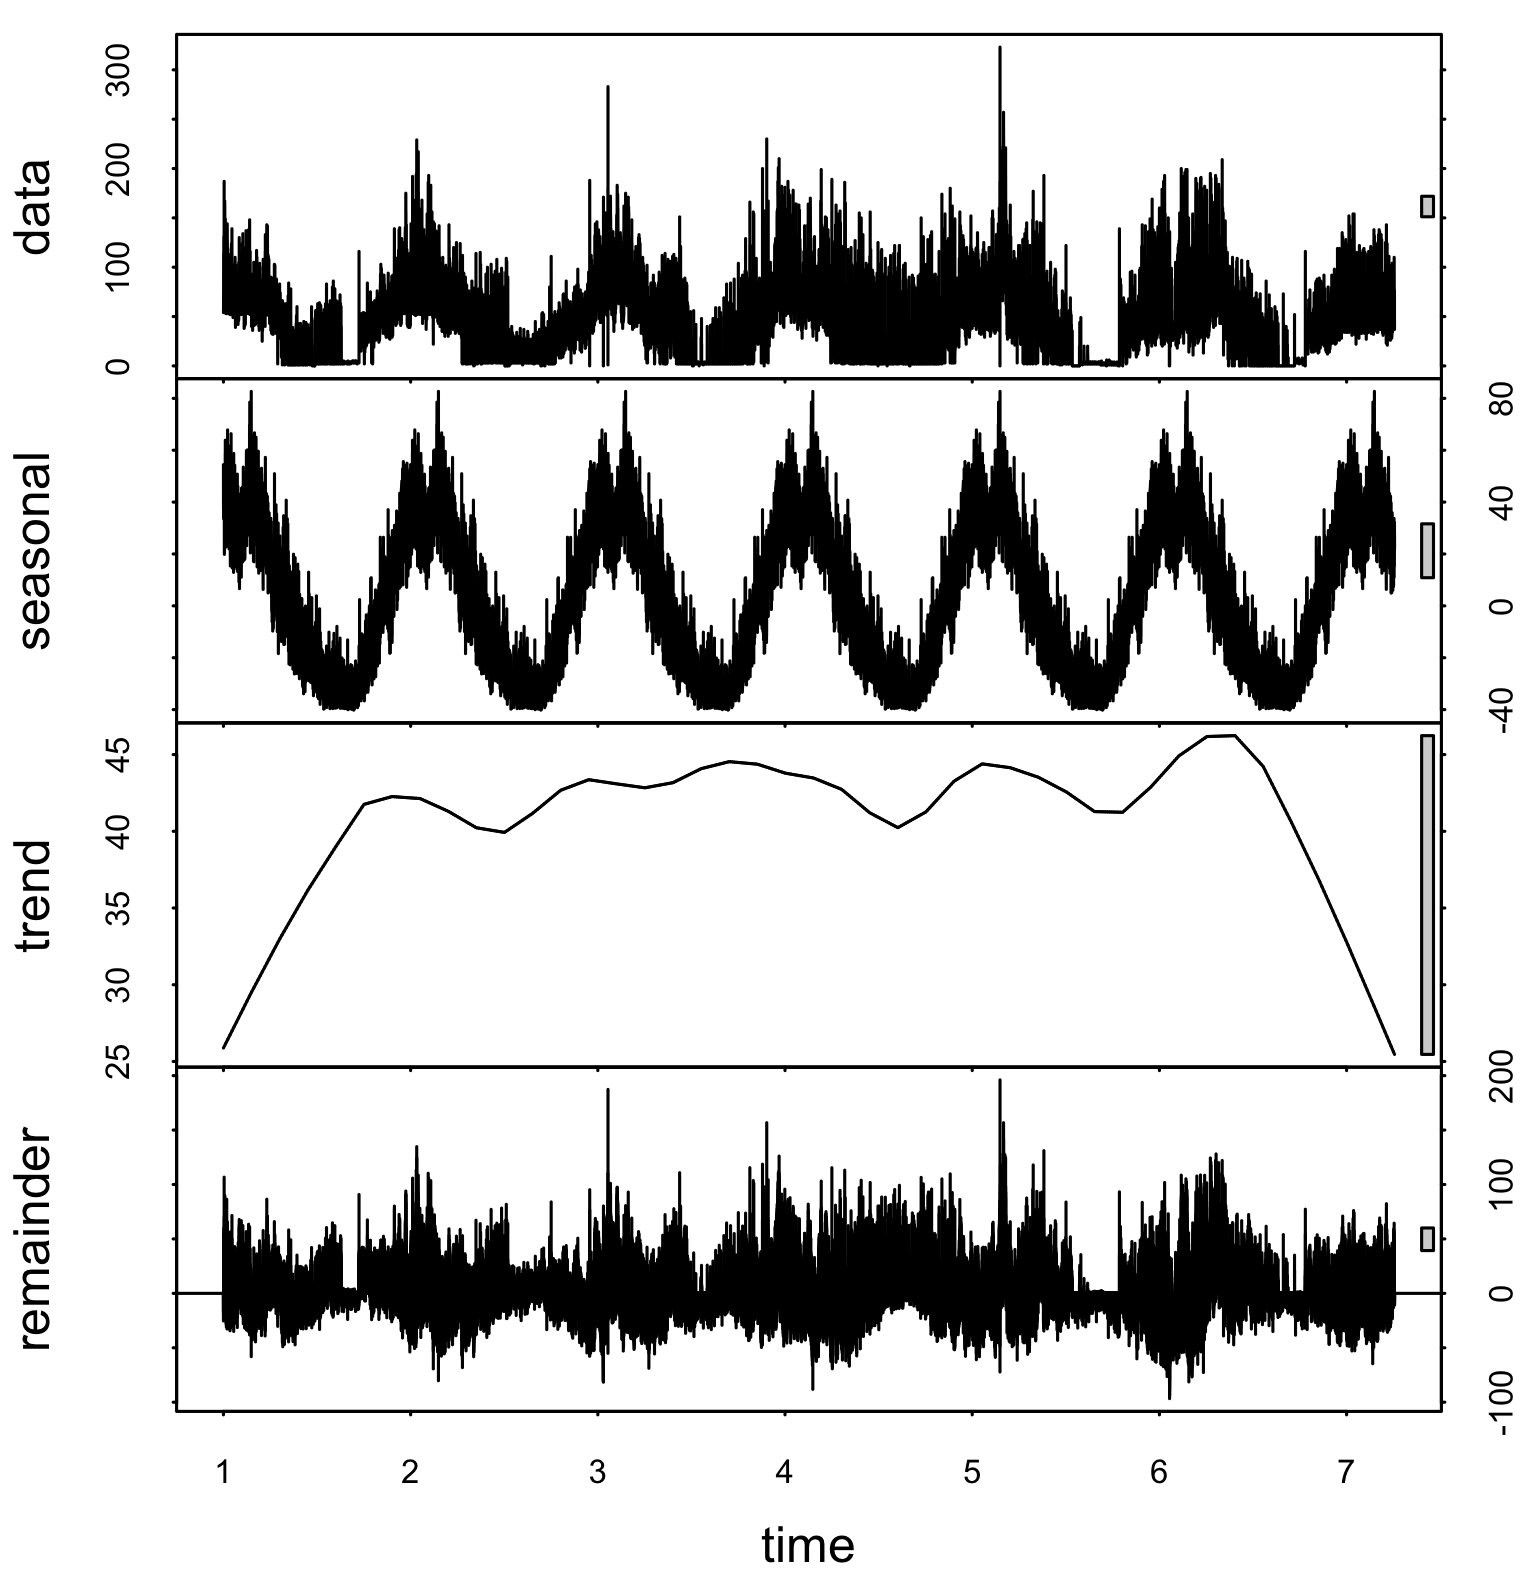
\includegraphics[width=\columnwidth]{STL.png}
\caption{Yearly STL decomposition by LOESS}
\label{fig:STL}
\end{figure}

In Zhang et al \cite{zhang1998forecasting} it is stated that ANNs models really have advantages while dealing with a large amount of historical load data with non-linear characteristic, but the researchers neglected the linear relations including the data. For this reason a hybrid approach is proposed, where the ANN will be helped in linear forecasting by the popular method ARIMA (auto-regressive integrated moving averages), commonly known as the Box–Jenkins approach. In order to apply ARIMA, the time-series was processed iteratively with a moving window of $21$ days where the ARIMA model was fitted. After the fitting it was forecasting the values of the next $24$ hours, before moving the window and doing the same for the day after. The seasonal ARIMA fitting was done by the help of the Forecast R package \cite{hyndman2007automatic} and its \emph{auto.arima} method, which finds the best ARIMA $(p,d,q) (P,D,Q)_m$ parameters by comparing the \emph{Akaike information criterion} (AIC) of the tested models. Just for the sake of the reader curiosity, the most fitted model was ARIMA $(3,0,3) (2,0,1)_{24}$. An ARIMA model with temperature dummy variables was tested, but it was not helping further the ANN: the simplest models was preferred.

Taking into account the points made in this section, the ANN is predicting the gas consumption ``seeing" without knowing its shape, and its behaviour in the previous hours/days. This limit is surpassed by some rolling windows, which will somehow simulate the Recurrent neural networks behaviour. Two rolling windows were created for the gas consumption, memorizing the sum and the peak load of the previous five hours, and two moving rolling windows were created for the STL yearly residuals, memorizing sum and peak of them.

All the features that were not between the limits $[-1,1]$ were scaled to have a faster convergence \cite{lecun2012efficient} of the \emph{Stochastic Gradient Descent} (\cref{eq:scaled}).
\begin{equation}\label{eq:scaled}
x'_i=\frac{x_i -  \frac{max(x) + min(x)}{2}}{ \frac{max(x) - min(x)}{2}}\end{equation} where $x_i$ is the original value and $x'_i$ is the scaled one. Many practical tricks like the shuffling of the elements, the normalization and initialization were taken from \cite{lecun2012efficient, bottou2012stochastic}.

All the process described so far is also called \emph{feature engineering} and was done almost iteratively, cumulatively introducing and removing features from the model and comparing the performance.

\begin{table}
\centering
\caption{ANN inputs}
\label{tab:ANNinputs}
\begin{tabular}{ll} \hline
Variable			& Data\\ \hline
Electricity load 		& $E(t)$ \\ 
Hour				& $sin(2\pi(h)/24)$; $cos(2\pi(h)/24)$\\
Week day			& $sin(2\pi(wDay)/6)$; $cos(2\pi(wDay)/6)$ \\
Month			& $sin(2\pi(mon)/12)$; $cos(2\pi(mon)/12)$ \\
Year day			& $sin(2\pi(d)/366)$; $cos(2\pi(d)/366)$ \\
Gas peak load$'$	& $\max_{1 \leq k \leq 5}G(t-k)$ \\
Gas sum load$'$	& $\sum_{i=1}^{5} G(t-i)$ \\
Gas mean load$'$	& $\frac{1}{288}\sum_{i=1}^{288} G(t-i)$ \\
Temperature		& $T(t)$ \\
Wind speed		& $FH(t)$ \\
$\Delta T_{k+1}$	& $T_{k+1} - T_{k}$ \\
ARIMA forecast		& $forecast(\operatorname{ARIMA} (3,0,5), 1)$ \\
STL year res.		& $YearRes(t)$ \\
STL weekly res.		& $WeeklyRes(t)$ \\
STL day res.		& $DayRes(t)$ \\
Year res. peak		& $\max_{1 \leq k \leq 5} YearRes(t-k) $ \\
Year res. sum		& $\sum_{i=1}^{5} YearRes(t-k)$ \\
STL T res.			& $Res(T(t))$ \\
STL FH res.		& $Res(FH(t))$ \\
STL E res.			& $Res(E(t))$ \\
\hline
\end{tabular}
\end{table}

Choosing number of hidden units for the ANN is always a tricky task. As stated by \cite{lawrence1998size, sarle1995stopped}, using \emph{early stopping} in a oversized \emph{Backpropagation} ANN, where the number of hidden neurons is higher than the number of the features, makes easier to find global optimum and avoid bad local optima. For this reason the number of hidden units was chosen to be greater than $2\times |features|$ and then test-driven and the training was early stopped to prevent \emph{overfitting}.

\subsubsection{Architecture}

ANNs are trained trying to minimize a cost function of the form
\begin{displaymath}E= \frac{1}{N}\sum_{i=1}^np(r_i)^2\end{displaymath}
where the error function $p$ is symmetric and continuous, $r_i = Y_i - \hat{Y_i}$ is the residual between the actual value and the forecast one, and $N$ is the number of training patterns.

Using the notations defined above, the most used cost function is based on the Mean Squared Error (MSE), commonly known in data modelling as Least Mean Squares (LMS) method. The basic idea of LMS is to optimize the fit of a model with respect to the training data by minimizing the square of residuals
\begin{displaymath}p(r)= \frac{1}{2}r^2\end{displaymath}
but it is greatly influenced by outliers \cite{liano1996robust}. In order to control the damage caused by outliers, in this paper the Least Mean Log Squares (LMLS) method presented by \cite{liano1996robust} is used. It is defined in (\cref{eq:LMLS}).
\begin{equation}
p(r) = \log(1 + \frac{1}{2}r^2)
\label{eq:LMLS}
\end{equation}

The ANN is a 1-hidden-layer \emph{Multilayer Feedfoward} ANN with a feedback structure, called \textit{Backpropagation}. This ANN is composed by \emph{Rectifier} neurons and one output linear node. Training is done by the \emph{Stochastic Gradient Descent} algorithm with $10$ batch size and is characterized by a learning rate of $0.003$ and fixed by a Momentum of $0.05$, which could help to increase the speed, avoiding local minima.

\begin{figure}
\centering
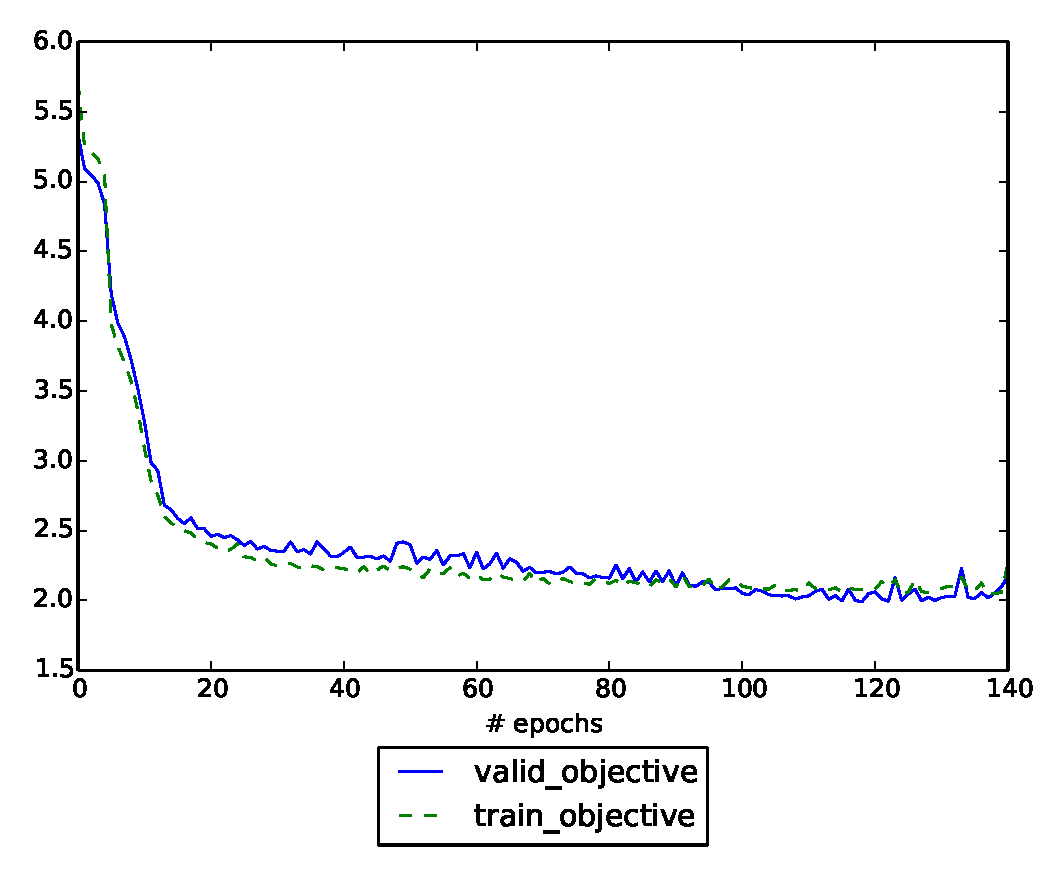
\epsfig{file=images/plot.eps, width=\columnwidth}
\caption{Training curve of the hybrid model with 80 hidden neurons}
\end{figure}

This project used Python and \emph{pandas} for the data analysis, \emph{Pylearn2} \cite{goodfellow2013pylearn2} to construct and test the ANN and the R system with the \emph{zoo} \cite{zeileis2005zoo} and the \emph{Forecast} \cite{hyndman2007automatic} packages for the ARIMA process. 


\subsection{Outlier detection}

According to Chebschev's theorem \cite{amidan2005data}, almost all the observations in a data set of system states falls into the interval $[\mu - 3\sigma, \mu+3\sigma]$, where $\mu$ and $\sigma$ are respectively the mean and standard deviation of the data set, and the data points outside this interval are declared outliers. In this paper the ANN is used to predict the gas consumption, for this reason a point will be considered outlier if it will fall outside the $95\%$ confidence interval\footnote{For the following description user \textit{fabee} of \emph{CrossValidated} needs to be mentioned: \url{http://tinyurl.com/l9gvz65}. } expressed for the RMSE. If it is assumed that the difference between the actual values $x_i$ and the predicted value $\hat{x_i}$ have:
\begin{equation}
\hat{x}_{i}-x_{i}	\sim	\mathcal{N}\left(0,\sigma^{2}\right)
\end{equation}
\begin{itemize}
\itemsep0em
  \item mean zero.
  \item follow a Normal distribution (it is assumed that it holds for the large amount of data utilized).
  \item and all have the same standard deviation $\sigma$.
\end{itemize}
\begin{equation}
\label{equation:preRMSE}
\hat{x}_{i}-x_{i}	\sim	\mathcal{N}\left(0,\sigma^{2}\right)
\end{equation}
it is possible to say that \cref{equation:preRMSE} follows a $\chi_{n}^{2}$ distribution with $n$ degrees of freedom. Which means:
\begin{align}
P\left(\chi_{\frac{\alpha}{2},n}^{2}\le\frac{n\mbox{RMSE}^{2}}{\sigma^{2}}\le\chi_{1-\frac{\alpha}{2},n}^{2}\right)	=	1-\alpha\\
\Leftrightarrow P\left(\frac{n\mbox{RMSE}^{2}}{\chi_{1-\frac{\alpha}{2},n}^{2}}\le\sigma^{2}\le\frac{n\mbox{RMSE}^{2}}{\chi_{\frac{\alpha}{2},n}^{2}}\right)	=	1-\alpha\\
\Leftrightarrow P\left(\sqrt{\frac{n}{\chi_{1-\frac{\alpha}{2},n}^{2}}}\mbox{RMSE}\le\sigma\le\sqrt{\frac{n}{\chi_{\frac{\alpha}{2},n}^{2}}}\mbox{RMSE}\right)	=	1-\alpha.
\end{align}
Therefore
\begin{equation}
\left[\sqrt{\frac{n}{\chi_{1-\frac{\alpha}{2},n}^{2}}}\mbox{RMSE},\sqrt{\frac{n}{\chi_{\frac{\alpha}{2},n}^{2}}}\mbox{RMSE}\right]
\end{equation}

\section{Experimental Evaluation}
The ANN has been trained with early stopping, with a fixed number of training epochs (phases) or stopping the training when the validation error rate was increasing. All the results showed are obtained from a k-fold cross-validation techniques, where the network was trained $k$ times, each time leaving out a subset of data from training in order to test the ANN. The results of the $k$ tests, were divided by $k$. The network is always trained with $70\%$ of the data, $15\%$ is used for validation and the other $15\%$ for testing.

Although most the Mean Absolute Percentage Error (MAPE) is considered a standard for examining the quality of the models prediction of energy load, it is an adequate error measure only if the loss function were linear and recent studies demonstrated it is not \cite{kalogirou2006artificial}\cite{kajl2000evaluation}. Moreover the percentage error is infinite if there are zero values on the series, frequent in intermittent data and in consumption data, and it puts a heavier penalty on positive errors than on negative errors \cite{hyndman2006another}. Because of these disadvantages, this paper will only consider the minimization of the Root Mean Square Error (RMSE), which penalize large errors, as suggested in \cite{yao2005method}. As suggested in \cite{hippert2001neural}, for every experiment also the Mean Absolute Error (MAE) will be calculated. 

\begin{equation}\operatorname{MAPE}\footnote{MAPE errors will be calculated only on the non-zero values, to avoid the problems described before.}=\frac{1}{n}\sum_{i=1}^{n} \frac{|Y_{i} - \hat{Y_i}|}{Y_{i}} \times 100 \end{equation}

\begin{equation}\operatorname{RMSE}=\sqrt{\frac{1}{n}\sum_{i=1}^n(\hat{Y_i} - Y_i)^2}\end{equation}

\begin{equation}\operatorname{MAE}=\frac{1}{n}\sum_{i=1}^n \left| \hat{Y_i}-Y_i\right|\end{equation}

\noindent where $\hat{Y}$ is the vector of the $n$ predictions and $Y$ is the vector of the true values.



\subsection{Synthetic experiments}
The method is tested with synthetic generated data. Two days outliers were generated by different algorithms. In the first one the real consumption was modified by a random value, simulating the system measurement/control malfunction which makes the consumption bouncing up and down (see \cref{equation:synt1}). The second synthetically created day was created adding $50 m^3$ of gas consumption to the real one, creating a pattern which simulates a strange behaviour and/or a malfunction of the heating system (see \cref{equation:synt2}).

\begin{equation}G(t)= G(t)+v*30\label{equation:synt1} \end{equation}
where 
\begin{align*}v \sim \mathcal{N} (0,\sigma^2) \end{align*}

\begin{equation}G'(t)= G'(t)+50\label{equation:synt2} \end{equation}

\begin{figure*}
\centering
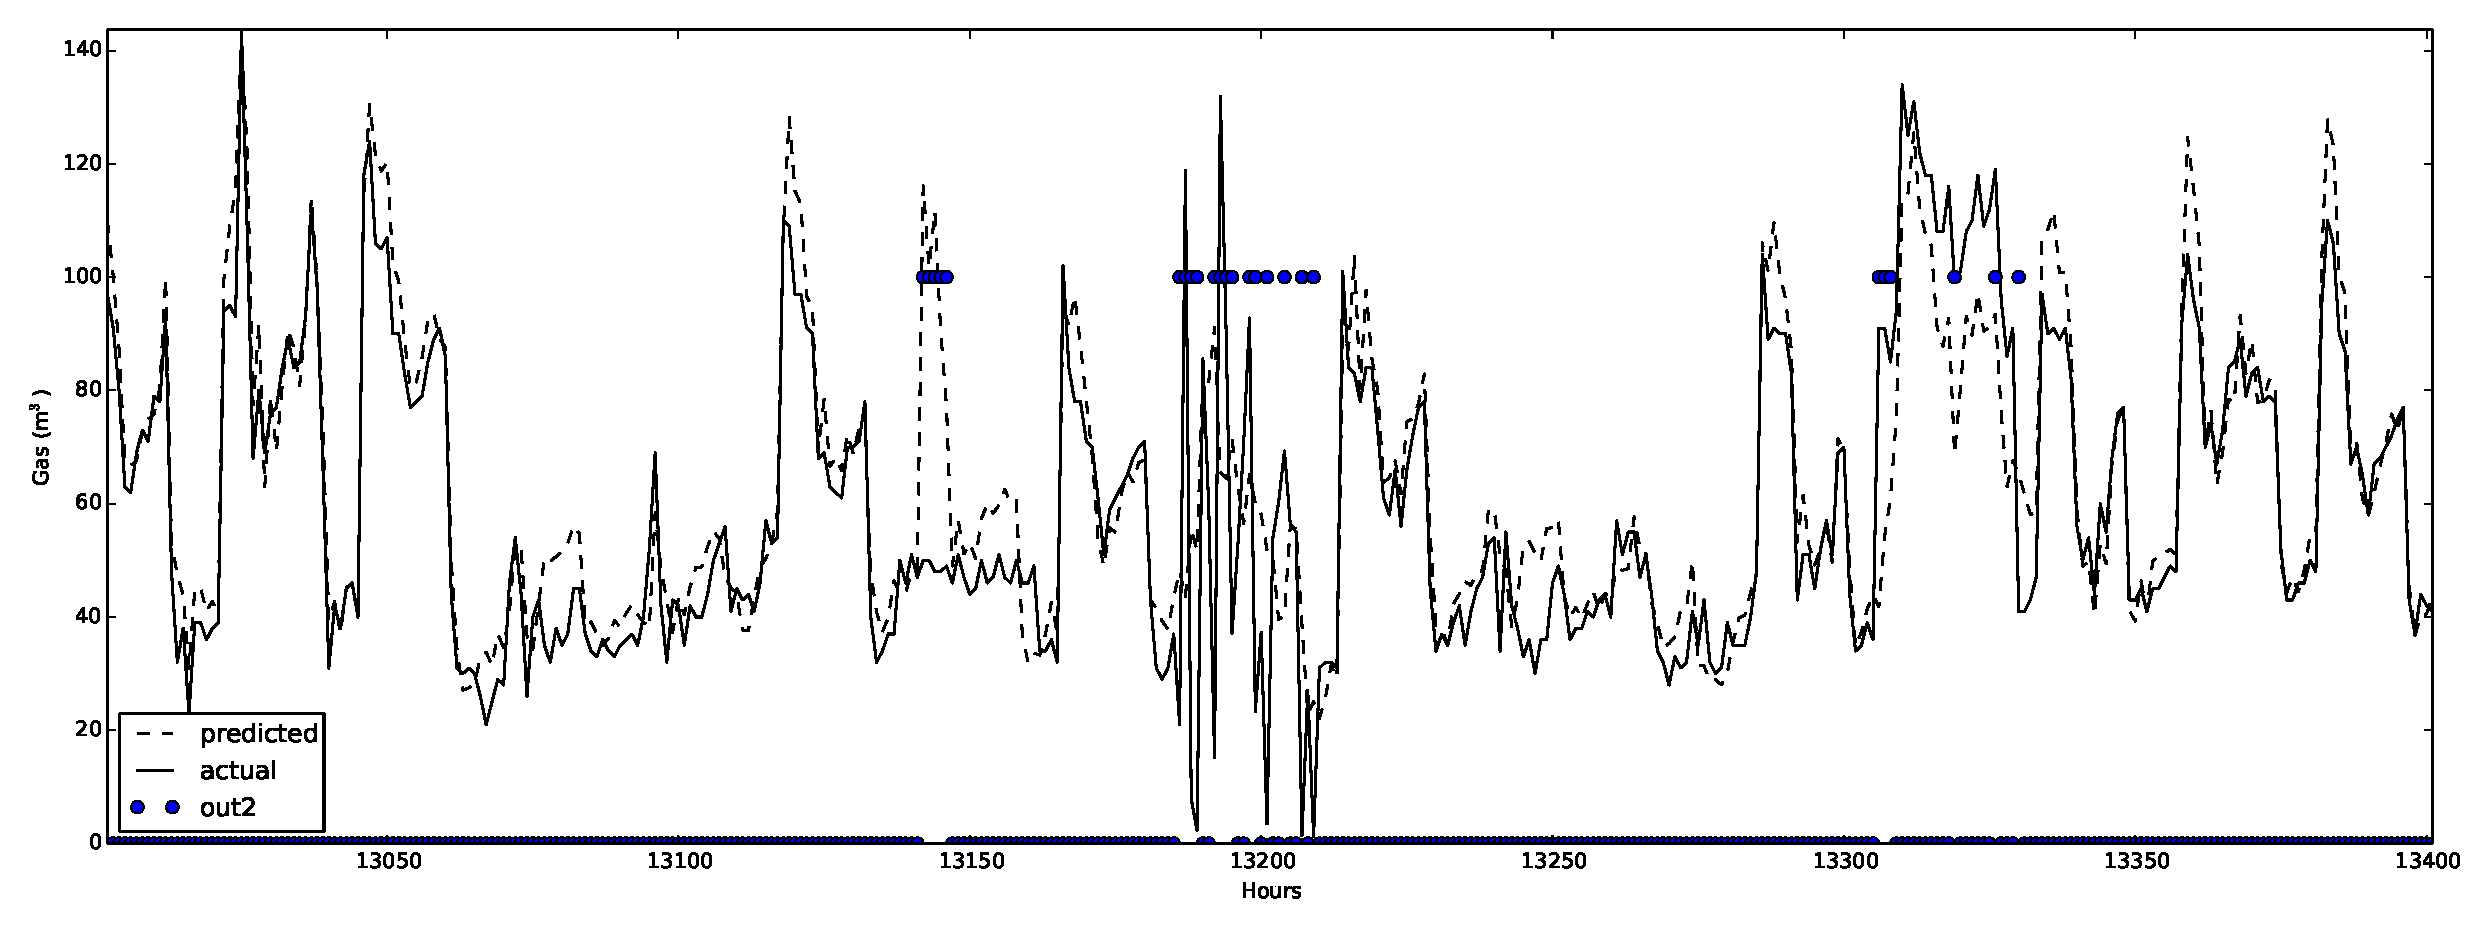
\includegraphics[width=\textwidth]{images/outliersSynt.eps}
\caption{Outlier detection with synthetic generated data. The circle represents the hours where an outlier is detected.}
\label{fig:outlierSynt}
\end{figure*}

The two outliers were correctly detected, as it can be seen in \cref{fig:outlierSynt}.


\subsection{Measured data experiments}
The method is also tested with measured data, coming from a different type of the day. For example the gas consumption of a week-end was placed in a week-day, simulating a holiday. The purpose of this test was to show that the unusual pattern was detected. In \cref{fig:outlierReal} it can be seen that the outlier mechanism works perfectly when the Sunday gas consumption is placed in a weekday. 

\begin{figure*}
\centering
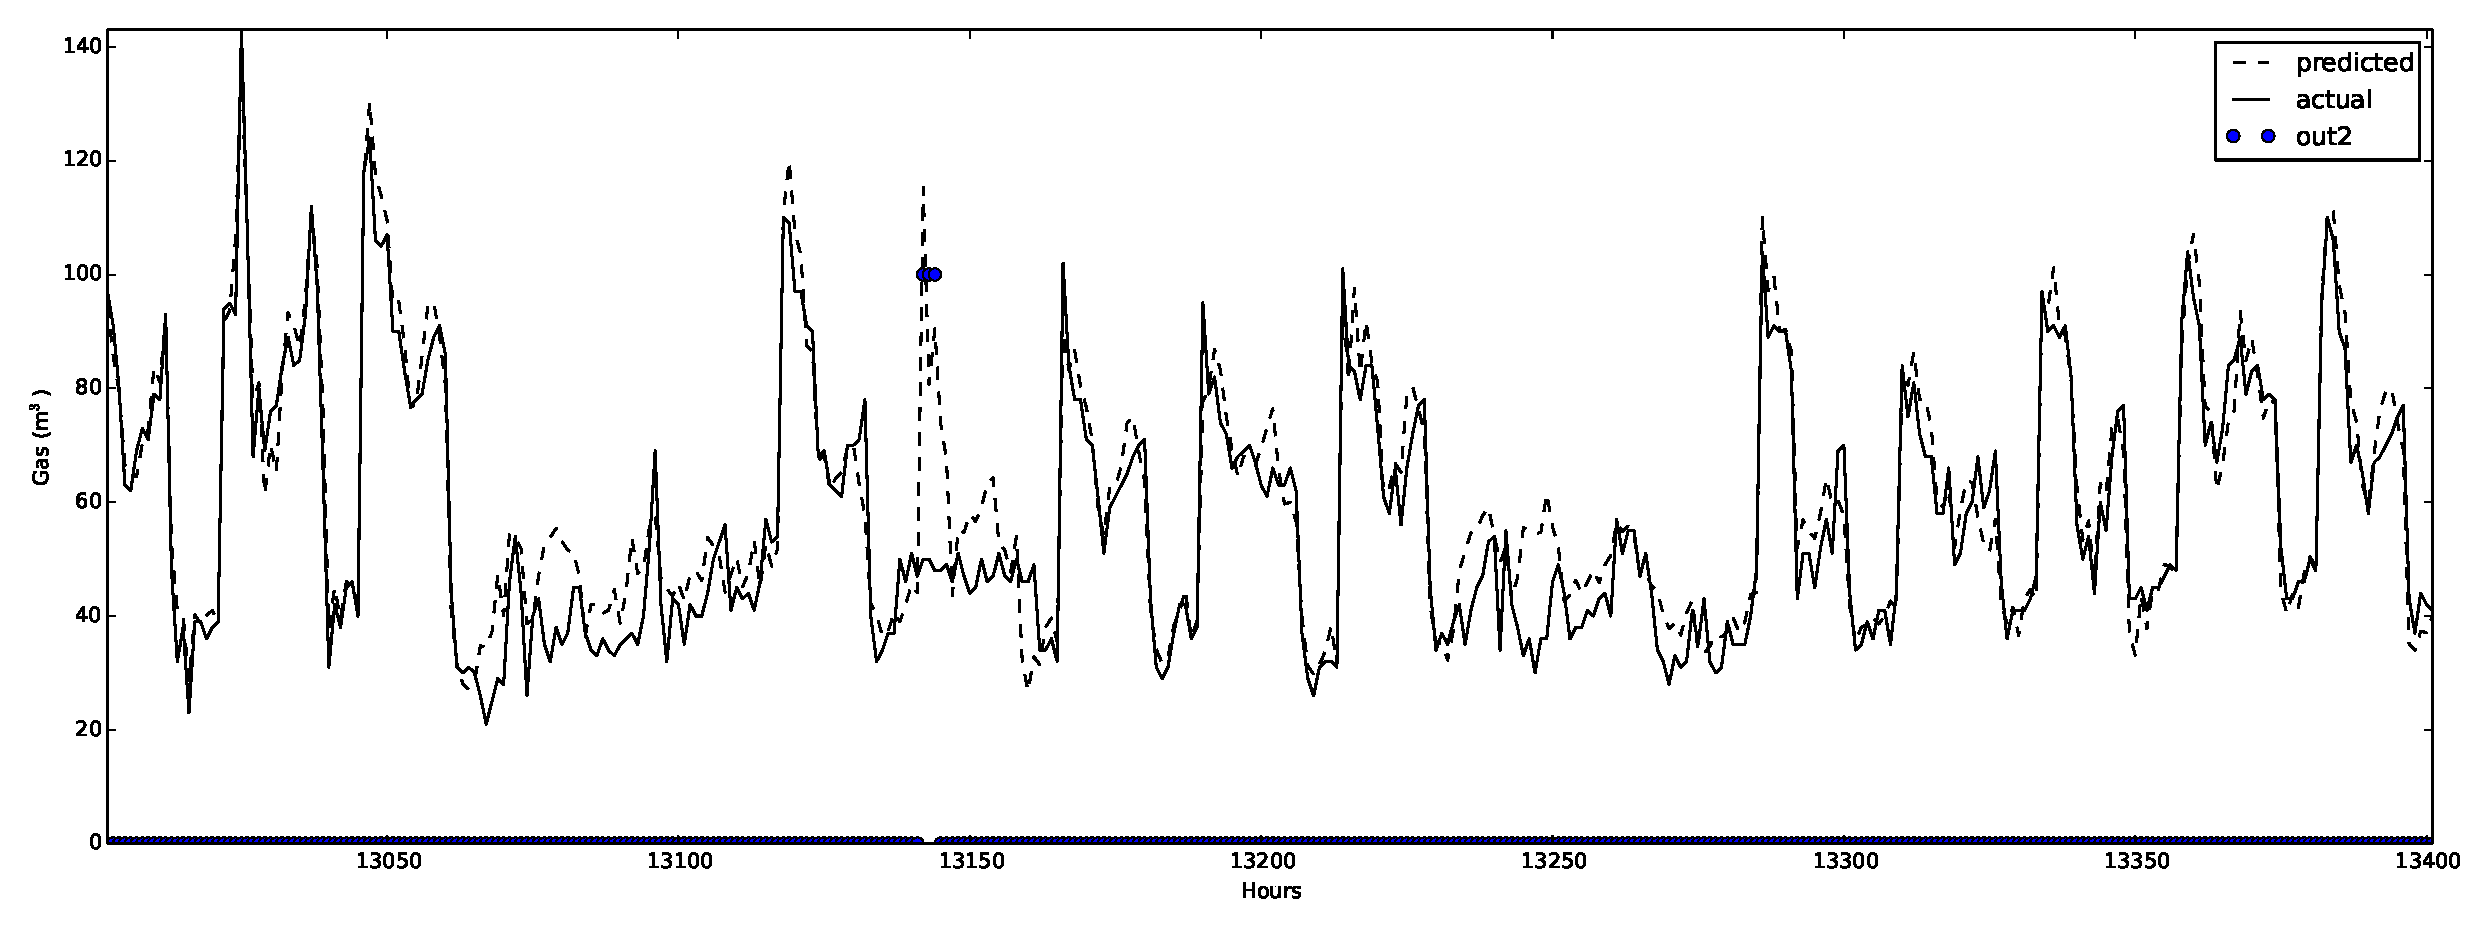
\includegraphics[width=\textwidth]{images/outliersReal.eps}
\caption{Outlier detection where the gas consumption of a weekday was replaced by a Sunday one. The (three) circles represent the outliers detected by the system.}
\label{fig:outlierReal}
\end{figure*}

The outlier was correctly detected, as it can be seen in \cref{fig:outlierReal}. The robustness of the design was proved with different building, listed in \cref{tab:dataset}.


\section{Future work}

ARIMA models can't detect more than one seasonality but it can be helped with Fourier terms and ARIMA \emph{dummy variables} to pro­duce rea­son­able fore­casts. When multi-seasonality is present, an algorithm like TBATS can overpass the ARIMA one, detecting it. This non-parametric model described in \cite{de2011forecasting} could be substituted to the ARIMA one as feature of the ANN. At the moment it is very slow, but it is very recent, so it will be probably improved.

The daily pattern could be seen in the transformed Fourier space applying the Modified Discrete Cosine Transform (MDCT) \cite{malvar1992signal}. In theory this could help as well to understand the pattern, but it was only applied once by  \cite{busseti2012deep}, with scarce results.

ANNs are sensitive to missing values and irregularities, but it was not possible to contact the buildings managers in order to possibly confirm/identify previously known outliers. For this reason the ANN training was done with not entirely perfect data, and this probably affected the performance. It is necessary to contact these building managers to further help the training of this algorithm. \\
The input variables were scaled standardizing them to a midrange 0 and range $[-1, 1]$. It is also possible to normalize them to have mean 0 and standard deviation 1. In this case Robust estimates of location and scale are desirable if the inputs contain outliers. Some examples are \cite{iglewicz1983robust} and the recent \cite{mizera2004location} can be the base of a future refine of the ANN inputs.


Before 2006, ANN were almost always associated with the \emph{Backpropagation} algorithm and with the 1-hidden layer architecture. The problem with these architectures is that they get stuck in poor local-optima. In 2006 there was a huge breakthrough mainly started by \cite{hinton2006fast}, which is called \emph{Deep learning} and it represent the new fashion of ANNs, based on multi hidden layers and new algorithms. \\
Future improvements can be based on Recurrent Neural Networks (RNNs) and Restricted Boltzmann Machines (RBMs) which were recently proved to be interesting in time-series forecasting \cite{busseti2012deep, taylor2009factored, sutskever2013training}. The \emph{Pylearn2} \cite{goodfellow2013pylearn2} RNN framework is under development.


\section{Conclusion}

Some interesting behaviours were found though this work:
\begin{description}
\itemsep0em
  \item[Holidays] Regardless of whenever the school was operational, the first tests showed that the Ebatech system was normally heating the buildings (Christmas, in Tuesday 25th of December 2012, was heated like a normal Tuesday even if the building was certainly closed). This causes an avoidable waste.
  \item[Consumption bounces] In \cref{fig:zigzag} a strange zig-zag behaviour can be seen. It seems that the system is wasting energy and this shape is totally different from the usual one (\cref{fig:dailyBehaviour}). This lasts for months and it is clear that also the ANN training is affected by this outlier-like behaviour.
\item[Peaks] Around the initial days of September there is a huge bounce of the consumption (up to three times more than the maximal consumption of the year). Is it a test?
\item[August with heaters] In August 2009 and August 2011 the heaters were active even with not apparent cold summer.
\item[Outliers] Some other outliers are found but they need to be confirmed by the managers, hopefully after the verification of the previously mentioned behaviours.
\end{description}
All these problems will be immediately reported to the company.

\begin{figure}[h!]
\centering
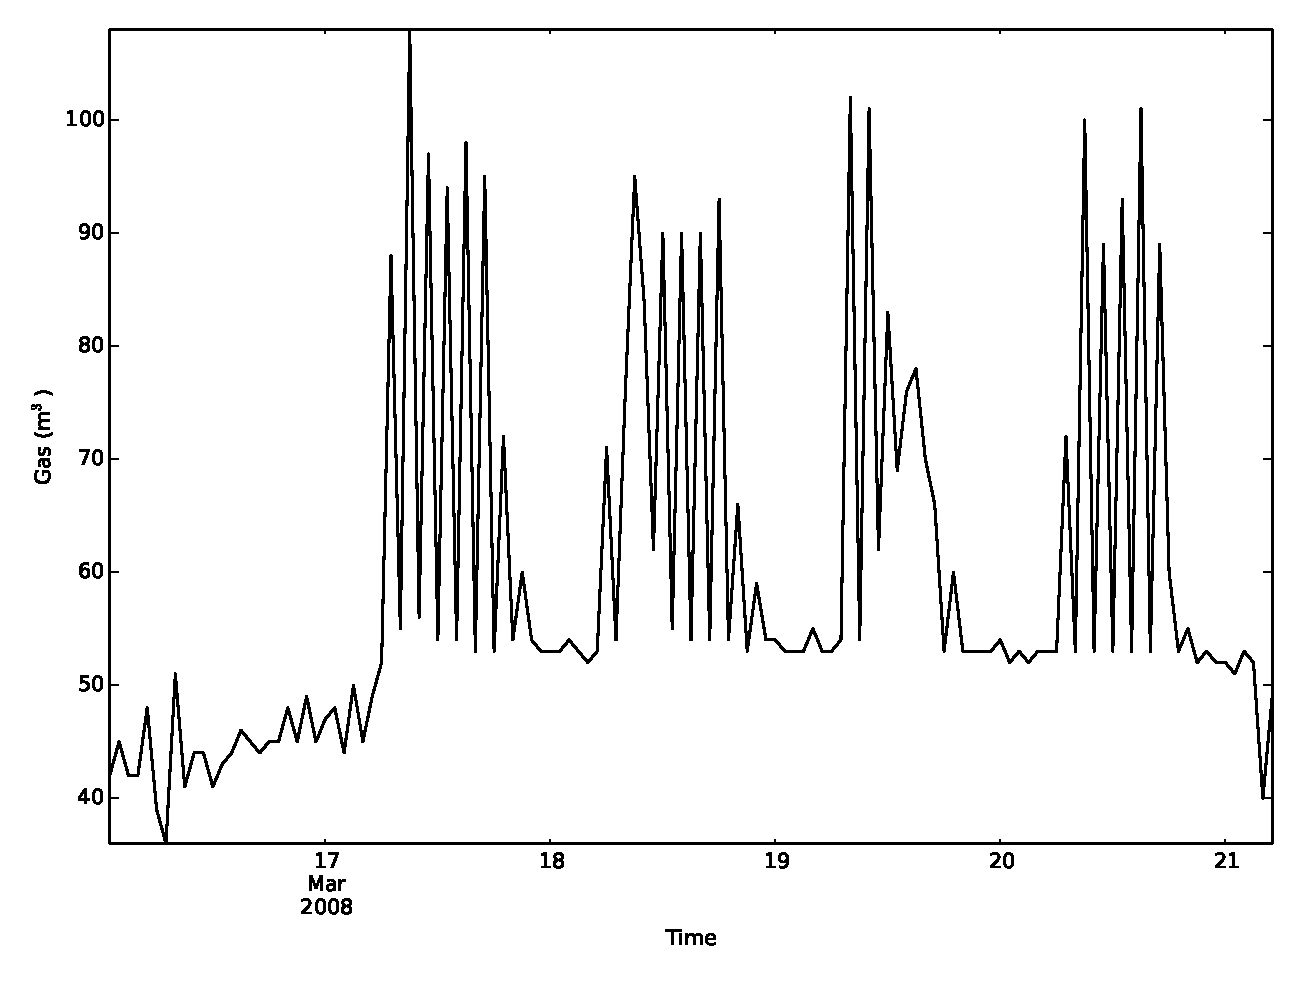
\epsfig{file=images/zigzag.eps, width=\columnwidth}
\caption{Strange zig-zag behaviour found by the algorithm.}
\label{fig:zigzag}
\end{figure}

An ANN with the standard cost function MSE was also trained, apparently resulting in a smaller RMSE error in a faster way (\cref{tab:ANNresults}). Although this can be true, the Hybrid LMLS model was more precise, detecting better the possible outliers. They contributed the most to the error.

\begin{table}
\centering
\caption{Best selected results to compare the ARIMA, ANN and hybrid model. HyMSE is the Hybrid model with MSE cost function, while HyLMLS is the same model with LMLS cost function.}
\label{tab:ANNresults}
\begin{tabular}{llllll} \hline
Model			& neurons & epochs \tablefootnote{epochs to converge} & RMSE & MAPE & MAE \\ \hline
ARIMA\tablefootnote{Calculated iteratively as described in \cref{sec:predictor}}			& - & - & 88.50 & 117.27  & 22.52  \\ 
ANN 				& 80 & 15 & 11.95 & 34.78  & 8.52 \\ 
HyMSE			& 80 &  70 & 9.4 & 27.66 & 6.90 \\ 
HyLMLS			& 150 & 140 & 10.02 & 30.05 & 7.26 \\ 
\hline
\end{tabular}
\end{table}

Any model can't be treating accurately all the situations for a large amount of historical load data. The irregular fluctuation of the gas consumption was hardly predictable, for this reason the ANN model was helped with robust cost function and with the well known ARIMA model. Although other papers presented similar models to forecast electric consumption, the hybrid model presented here, is almost unique because it focuses to forecast short-term gas consumption, which are very irregular and not easily predictable with classic methods. Since the predictor is very accurate (with RMSE of $10$ $m^3$), the outlier mechanism is able to easily detect strange behaviours defining a threshold value in the confidence interval without the need to possess previous examples of outliers. The scope of this paper was forecasting the highly irregular gas consumption time-series, but it is believed that similar results could be also obtained with electric consumption time-series. It is hoped that this could lead to new analysis of the energy consumption in public buildings.
\vfill

%\end{document}  % This is where a 'short' article might terminate


%ACKNOWLEDGMENTS are optional
\section{Acknowledgments}
This internship was economically supported by Universita' degli studi di Trento. I also thank Jesse Eisses who through his work helped me to find some interesting ideas for this paper.

%
% The following two commands are all you need in the
% initial runs of your .tex file to
% produce the bibliography for the citations in your paper.
\bibliographystyle{abbrv}
\bibliography{sigproc}  % sigproc.bib is the name of the Bibliography in this case
% You must have a proper ".bib" file
%  and remember to run:
% latex bibtex latex latex
% to resolve all references
%
% ACM needs 'a single self-contained file'!
%
%APPENDICES are optional
\appendix
%Appendix A
\section{Sources}
``Very often scientific studies rely on complex textual explanations of what has been done to analyse the data that can overwhelm the reader that has to accept them as an act of faith", as stated in \cite{reproducibility}. To avoid this, the author provides all the sources through this website: \url{https://github.com/denadai2/energyUva}. Some sources are also available for the popular Pybrain \cite{schaul2010} library.

The raw data are protected by privacy of the Hogeschool van Amsterdam. The Universiteit van Amsterdam is working to make them available to achieve total reproducibility.

%\balancecolumns

\balancecolumns % GM July 2000
% That's all folks!
\end{document}
